\chapter{State of the Art: Market Analysis}

\section{Industry Overview and Market Potential}

Drones are transforming agriculture by offering innovative solutions to enhance efficiency and sustainability. As reported by Chaundler in The New York Times \cite{chaundler2021}, companies like CO2 Revolution \cite{co2_revolution} are using drones to plant seeds in inaccessible areas, showcasing the potential of drone technology in reforestation and agricultural applications.

The global agricultural sector faces significant challenges, including the need to increase food production to meet the demands of a growing population and to address the impacts of climate change \citep{nazarov2023}. Traditional farming methods are often insufficient, leading to a surge in the adoption of drones for various agricultural purposes.

\subsection{Applications of Drones in Agriculture}

Drones are used in agriculture for a wide range of applications:

\begin{itemize} 
	\item \textbf{Crop Monitoring and Mapping:} Drones can provide high-resolution aerial imagery, enabling farmers to monitor crop health, identify pest infestations, and assess soil conditions in real-time \citep{nazarov2023, alliedmarketresearch2021}. 
	\item \textbf{Precision Spraying:} With precise positioning, drones can apply fertilizers, pesticides, and herbicides precisely where needed, reducing chemical usage and minimizing its environmental impact \citep{guardianagriculture, plantdiseasedetection2023}.
	\item \textbf{Irrigation Management:} Drones assist in detecting variations in soil moisture levels using thermal cameras, helping optimize irrigation systems and conserve water resources \citep{nazarov2023}. 
	\item \textbf{Planting and Seeding:} Some drones are designed to plant seeds over large areas efficiently, particularly useful in reforestation efforts and hard-to-reach terrains \citep{chaundler2021}. 
\end{itemize}

\subsection{Market Growth and Potential}

The agricultural drone market is experiencing significant growth. Valued at \$0.88 billion in 2020, it is projected to reach \$5.89 billion by 2030, with a compound annual growth rate (CAGR) of 22.4\% \citep{alliedmarketresearch2021}. Key factors contributing to this growth include:

\begin{itemize} 
	\item \textbf{Demand for Increased Food Production:} Global population growth drives the need for higher agricultural output, encouraging the adoption of efficient technologies like drones \citep{nazarov2023}. 
	\item \textbf{Technological Advancements:} Improvements in drone capabilities, such as enhanced sensors and longer flight times, make them more practical for agricultural applications \citep{guardianagriculture}. 
	\item \textbf{Adoption of Precision Farming Techniques:} Farmers are increasingly using drones for site-specific crop management to optimize resource use and increase yields \citep{alliedmarketresearch2021}. 
\end{itemize}

\subsection{Challenges and Opportunities}

While the potential is significant, the adoption of drones in agriculture faces several challenges:

\begin{itemize} 
	\item \textbf{Regulatory Barriers:} Strict government regulations on airspace and drone operations can hinder deployment \citep{nazarov2023}. 
	\item \textbf{High Initial Costs:} The expense of acquiring and maintaining advanced drones may be prohibitive for small-scale farmers.
	\item \textbf{Privacy and Safety Concerns:} The use of drones can raise privacy issues and pose safety risks to people and animals if not operated correctly \citep{petiole_drones_risks}. 
\end{itemize}

Our solution addresses these challenges by offering cost-effective drone tracking systems that reduce initial costs by eliminating the need for expensive onboard navigation systems. By utilizing ground-based tracking, the drones used for our system can be simpler and more affordable, enhancing operational safety and accessibility for small-scale farmers. Moreover, we can leverage government support initiatives like Austria's "Smart Farming" action plan, which provides funding and resources to integrate digital technologies into agriculture \citep{smartfarming2023}. Additionally, implementing privacy and safety features such as geofencing and privacy-by-design principles ensures compliance with regulations and builds trust among users \citep{secure_redact_drones_privacy}.

\section{Target Group Definition}

Our ideal customers are small to medium-sized agricultural enterprises, individual farmers, and agricultural cooperatives with limited budgets. They seek cost-effective solutions to modernize their farming operations with drone technology without the high expenses associated with advanced onboard systems.

\textbf{Key Characteristics}

\begin{itemize}
	\item \textbf{Demographics}: Farmers and managers aged 35--60 with practical experience in agriculture, often fitting the "Progressive Realists" or "Adaptive-Pragmatic Middle Class" Sinus-Milieus  \cite{sinus_institut_2024}. 
	\item \textbf{Geographics}: Located in rural agricultural regions such as Lower Austria, Styria, Upper Austria, and Tyrol. 
	\item \textbf{Psychographics}: Value efficiency, sustainability, and are open to adopting new technologies that improve their farming practices. 
	\item \textbf{Behavioral}: Make purchase decisions based on cost-benefit analysis, attend local agricultural events, rely on recommendations from peers and local networks. 
	\item \textbf{Needs}: Affordable and reliable drone tracking systems that are easy to implement and help optimize farming operations. 
	\item \textbf{Technographics}: Moderate technological proficiency, use basic agricultural management tools, interested in user-friendly technology solutions. 
\end{itemize}

\section{Buyer Personas}

\textbf{Persona 1 (Core): Thomas Bauer}

\begin{itemize}
	\item \textbf{Age}: 52 
	\item \textbf{Role}: Owner of a medium-sized family farm 
	\item \textbf{Location}: Lower Austria
	\item \textbf{Goals}: Increase crop yields and operational efficiency through affordable technology 
	\item \textbf{Pain Points}: Limited budget for high-end drones; needs cost-effective tracking solutions that don't require extensive technical expertise
	\item \textbf{Behavior}: Reads local agricultural journals, attends regional farming expos, values practical and easy-to-use solutions 
\end{itemize}

\textbf{Persona 2 (Core): Maria Hofer}

\begin{itemize} 
	\item \textbf{Age}: 40 
	\item \textbf{Role}: Owner of a small organic farm 
	\item \textbf{Location}: Graz, Styria 
	\item \textbf{Goals}: Implement sustainable farming practices with the help of affordable technology 
	\item \textbf{Pain Points}: Needs reliable tracking solutions that align with organic farming principles; constrained by a tight budget 
	\item \textbf{Behavior}: Active in local farming communities, follows agricultural trends online, seeks eco-friendly and cost-effective solutions 
\end{itemize}

\textbf{Persona 3 (Peripheral): Andreas Schneider}

\begin{itemize} 
	\item \textbf{Age}: 55 
	\item \textbf{Role}: Manager of a farming cooperative 
	\item \textbf{Location}: Upper Austria 
	\item \textbf{Goals}: Enhance productivity for cooperative members through shared resources and technology 
	\item \textbf{Pain Points}: Finding affordable technology solutions that can be easily adopted by multiple farmers with varying levels of technical skill 
	\item \textbf{Behavior}: Engages with cooperative members, attends agricultural seminars, values solutions that offer collective benefits 
\end{itemize}

\section{Competitor Analysis}

The agricultural drone market in Austria and globally is highly competitive, with key players offering advanced precision farming solutions. This analysis focuses on three major competitors relevant to the Austrian market:

\begin{enumerate} 
	\item \textbf{Dronetech by Immotech (Austria):} Dronetech partners with Huawei to develop 5G-enabled smart farming drones. They modify DJI drones, already equipped with \acrfull{gnss}, \acrfull{rtk}, and obstacle avoidance cameras, adding custom \acrshort{3d}-printed parts to optimize them for agricultural needs \cite{dronetech_instagram, dji_m300}. Enhancements include high-resolution cameras and sensors, leveraging Huawei's cloud computing and \acrfull{ai} for real-time data analysis. This enables precise application of water, fertilizers, and pesticides, reducing waste and environmental impact. A key challenge they face is limited 5G network coverage \cite{huawei_dronetech_2022, huawei_boosting_farming_2022, dronetech_smart_farming_project}.
	
	\item \textbf{DJI - Da-Jiang Innovations Science and Technology Co. (China):} DJI, a global drone leader, offers expensive high-tech agricultural drones like Agras T50, T25, and Mavic 3M for tasks such as spraying, mapping, and crop monitoring. They use \acrshort{gnss} and \acrshort{rtk} for precise positioning, radar and vision sensors for obstacle avoidance, and Radio, Wireless Fidelity (WiFi), and Bluetooth for communication. Accessories like DJI Relay enhance their range in complex environments \cite{dji_ag_t25, dji_ag_t50}. In Austria, partners like Drohnenring distribute DJI's products, offering consultation, sales, training, and support \cite{drohnenring_2024}.
	
	\item \textbf{AgEagle Aerial Systems Inc. (United States of America (USA)):} AgEagle specializes in agricultural mapping drones like eBee X. Equipped with \acrshort{gnss} and \acrshort{rtk}, they achieve centimeter-level accuracy without ground control points. They communicate via radio links up to 3 km with secure encryption. Light Detection and Ranging (LiDAR) sensors provide obstacle avoidance and controlled landings. AgEagle offers software like eMotion and Measure Ground Control for flight planning and data processing \cite{ageagle_agriculture_2024, ageagle_agriculture_ebee}.
\end{enumerate}

\subsection{Competitive Landscape}

The Austrian agricultural drone market includes local firms like Dronetech, partnering with global tech companies, and international players like DJI and AgEagle, offering advanced drone technology and services. Competition centers on integrating cutting-edge technologies like 5G, \acrshort{ai}, \acrshort{gnss}/\acrshort{rtk} positioning, and advanced imaging to enhance precision farming. Competitors offer sophisticated communication systems, precise positioning, and advanced software solutions to meet modern agriculture's needs.

\subsection{Our Differentiation and Positioning}

\begin{figure}[H] 
	\centering 
	\hspace*{-1.5cm} 
	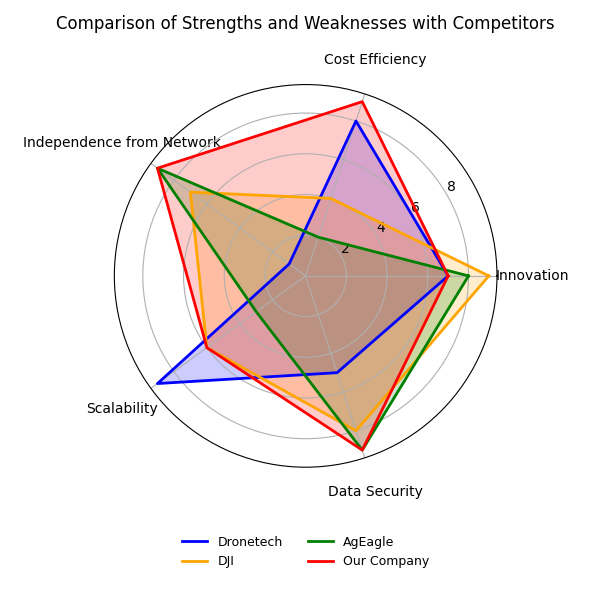
\includegraphics[width=400pt]{figures/competitors.png} 
	\caption{Comparison of strengths and weaknesses with competitors}
	\source{Own illustration created with Matplotlib in Python}
	\label{fig:strengths_weaknesses} 
\end{figure}

Our ground-based \acrshort{3d} drone tracking system offers an affordable and independent solution for Austria's agricultural sector. By using calibrated ground stations with advanced image processing, we eliminate the need for expensive onboard positioning and obstacle avoidance systems. This allows to deploy simpler drones, reducing costs, maintenance complexities, and payload restrictions. As a result, small to medium enterprises can access modern drone technology, overcoming challenges like network coverage limitations and high equipment costs, making it a practical tool for improving farming operations without substantial investment.

Our approach provides several key benefits:

\begin{itemize} 
	\item \textbf{Enhanced Efficiency and Cost Savings:} Without heavy onboard sensors, drones are lighter and consume less energy, thus increasing flight times and coverage area. They can carry more payloads like seeds, fertilizers, or pesticides, enhancing operational efficiency. Reduced complexity lowers maintenance and failure risk, leading to cost savings and making precision agriculture accessible to farmers with limited budgets.
	
	\item \textbf{Secure, Independent Communication:} Our local communication system operates independently of network infrastructure, ensuring reliability in areas with connectivity issues. Unlike competitors relying on 5G, our system enhances reliability, data security, and privacy by processing tracking data locally.
	
	\item \textbf{Scalability and Flexibility:} Our ground stations can track multiple drones simultaneously without adding complexity or weight to drones. This enables scalable operations, allowing farmers to expand fleets without significant additional investment.

\end{itemize}

\section{Conclusion}

The market analysis reveals a significant opportunity for our ground-based \acrshort{3d} drone tracking system in the agricultural sector. As drone adoption in agriculture accelerates, our solution addresses key challenges like high costs, dependence on network infrastructure, and the complexity of onboard systems by eliminating the need for expensive onboard positioning, and obstacle avoidance equipment. By enabling the use of simpler, more affordable drones with increased payload capacity and simplified maintenance, we offer a unique value proposition that differentiates us from competitors relying on complex onboard technologies. Our system aligns with the needs of small to medium agricultural enterprises seeking efficient and sustainable technologies without the barriers of high initial investment and technical complexity. Further research and engagement with industry stakeholders will refine our understanding of target customers and support a successful market entry, positioning us as a competitive player in the agricultural drone market focused on accessibility and practicality.
